%!TEX root = master.tex

\section{Policy gradient methods}
Policy gradient methods are a class of model-free reinforcement learning algorithms that directly optimizes the policy, maps the states to action by using gradient descent. By using gradient of the expected return with respect to the policy parameters, these class of methods iteratively updates the policy to improve the performance. 

\subsection*{Value-based vs Policy based RL}
The value-based RL methods are what we have looked at so far. Here we learn the value function and act greedily ($\epsilon$-greedy). In policy-based methods we don't use a value function, but learn a policy instead. In the next chapters we will take a look at Actor-critic methods were we learn the value function and policy.

\begin{figure}[ht!]
\centering
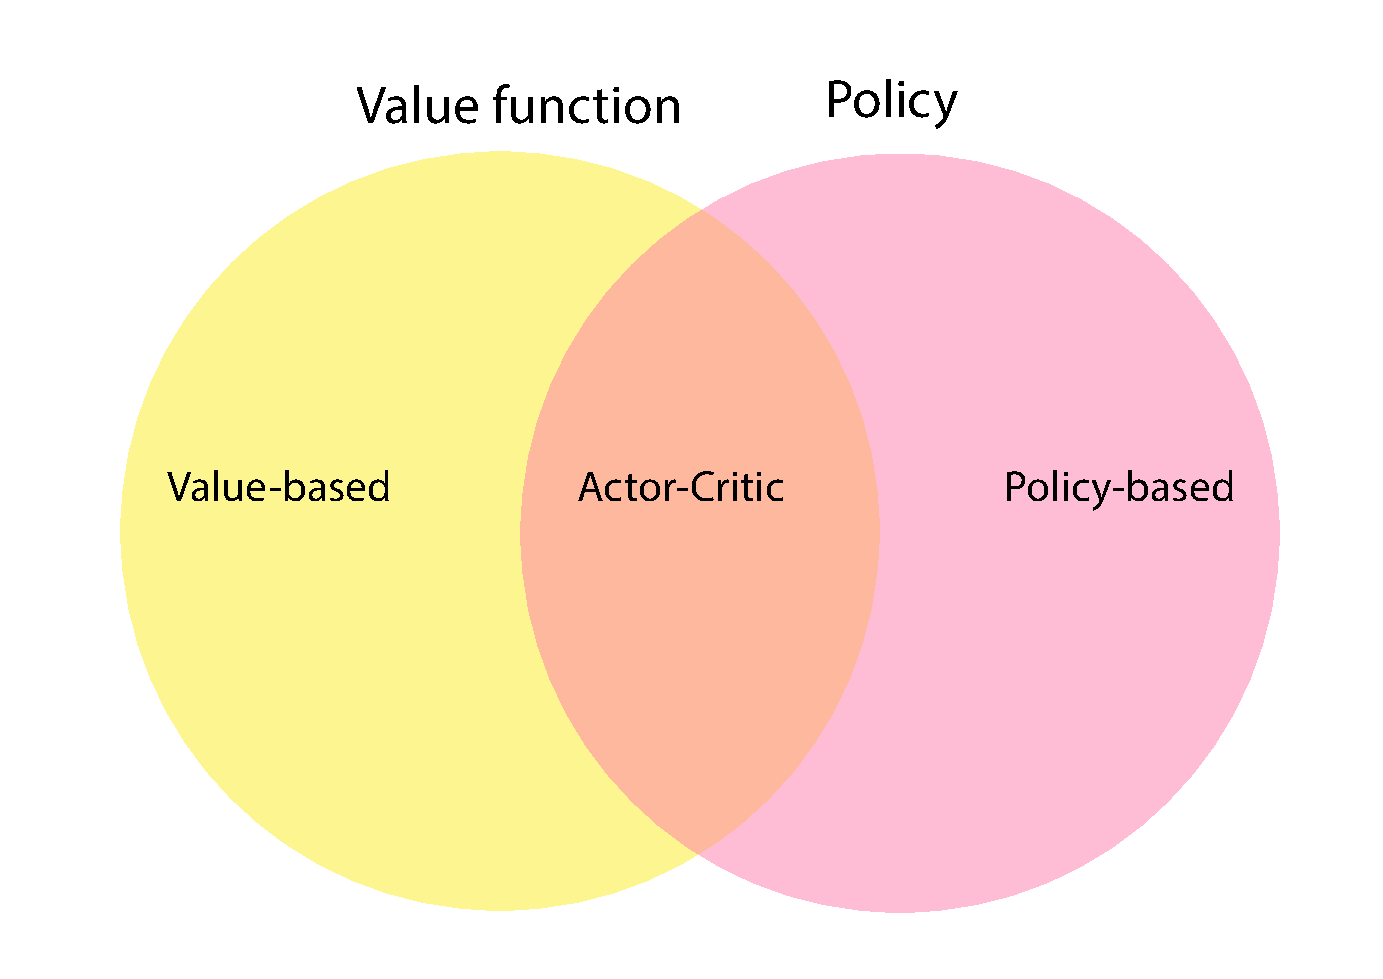
\includegraphics[width=80mm]{figures/valuepolicy.pdf}
\caption{Example of caption}
\label{fig:example}
\end{figure}


\subsection*{Policy based methods}
We parameterize the policy with some unknown parameters $\theta$ 


